%\documentclass[useAMS, usenatbib,usegraphicx,letter]{mn2e}
%\documentclass[11pt]{article}
\documentclass[reprint,aps,prd,superscriptaddress,showkeys,showpacs]{revtex4-1}
\usepackage{epsfig,amsmath,natbib}

\usepackage{aas_macros}
\usepackage{amssymb}
\usepackage{amsmath}
\usepackage{dsfont}
\usepackage{hyperref}
\usepackage{color}
\usepackage{pbox}
\usepackage{booktabs}

\hypersetup{
	colorlinks=false,
	citecolor=green
}
% \usepackage{graphicx}
% \usepackage{epstopdf}
% \usepackage{natbib}

%%%%%%%%%%%%%%%%%
%Custom commands%
%%%%%%%%%%%%%%%%%

\newcommand{\bb}[1]{\mathbf{#1}}
\newcommand{\bbh}[1]{\mathbf{\hat{#1}}}
\newcommand{\h}[1]{\hat{#1}}
\newcommand{\ttt}[1]{\texttt{#1}}

%%%%%%%%%%%%%%%%%%%%%%%%%%%%%%%%%%%%%%%%%%%%%%

\begin{document}

\title{Mocking the Weak Lensing universe: the LensTools computing package}

\author{Andrea Petri}
\email{apetri@phys.columbia.edu}
\affiliation{Department of Physics, Columbia University, New York, NY 10027, USA}
\affiliation{Physics Department, Brookhaven National Laboratory, Upton, NY 11973, USA}

\date{\today}

\label{firstpage}

\begin{abstract}
We present a newly developed software package which implements a wide range of routines frequently used in Weak Gravitational Lensing (WL). With the continuously increasing size of the WL scientific community we feel that easy to use APIs for common calculations are a necessity to ensure efficiency and coordination across different working groups. Coupled with existing open source codes, such as \ttt{CAMB}\citep{CAMB} and \ttt{GADGET2}\citep{Gadget2}, \ttt{LensTools} brings together a fully functional cosmic shear simulation pipeline which, coupled with a variety of WL feature measurement tools and parameter sampling routines, provides easy access to the numerics for theoretical studies of WL as well as for experiment forecasts. Being implemented in \ttt{python}\citep{python}, \ttt{LensTools} takes full advantage of a range of state--of--the art techniques developed by the large and growing open--source software community.    
    
\end{abstract}


\keywords{Weak Gravitational Lensing --- Simulations}
\pacs{98.80.-k, 95.36.+x, 95.30.Sf, 98.62.Sb}

\maketitle


%%%%%%%%%%%%%%%%%%%%%%%%%% INTRO %%%%%%%%%%%%%%%%%%%%%%%%%%%%%%%%%%%%%%%%%%%%%%%%%%%%%%%%

\section{Introduction}
%
Cosmology is entering a new, data driven era. After the Cosmic Microwave Background (CMB) (cite) provided one of the first experimental evidences of cosmological theories, a variety of different probes have been proposed to unveil the secret of the cosmos. Weak Gravitational Lensing uses the correlation between image distortions of background sources by Large Scale Structure (LSS) to infer cosmological parameters. Because... 

%%%%%%%%%%%%%%%%%%% CODE %%%%%%%%%%%%%%%%%%%%%%%%%%%%%%%%%%%%%%%

\section{Code} 

\subsection{Shear field simulations}

\begin{figure*}
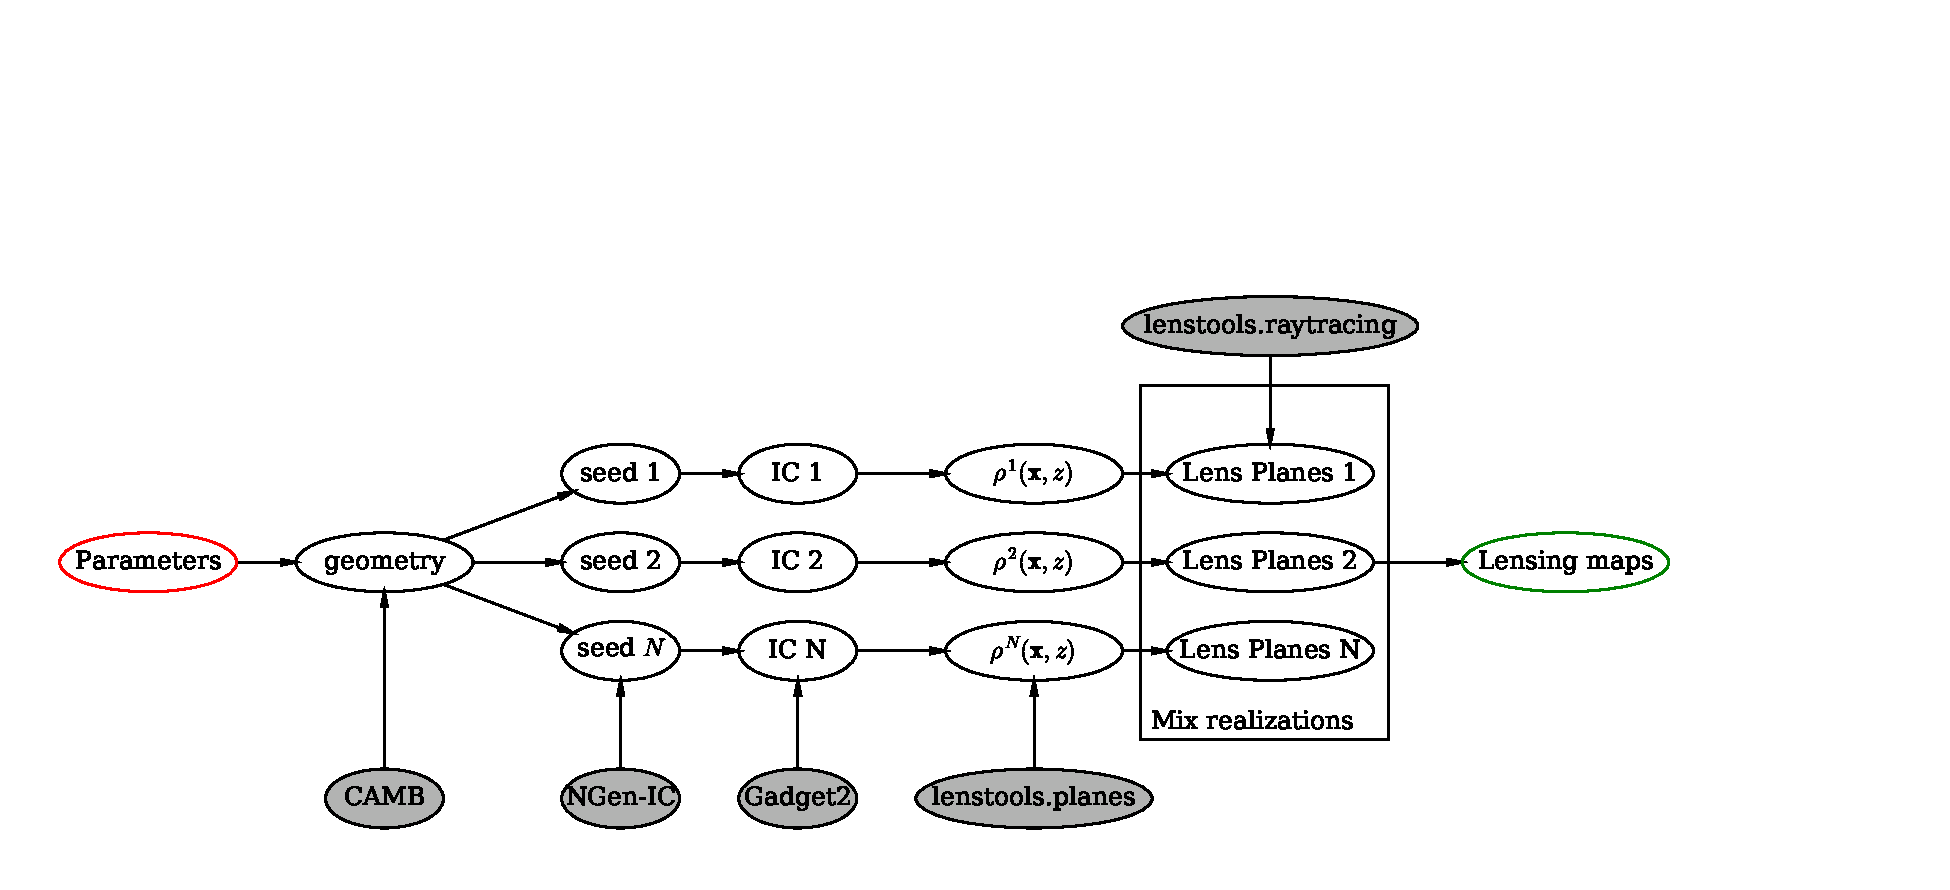
\includegraphics[scale=0.6]{Figures/flow.eps}
\end{figure*}



\subsection{Weak lensing features}

\subsection{Parameter estimation}

%%%%%%%%%%%%%%%%%%% EXAMPLES %%%%%%%%%%%%%%%%%%%%%%%%%%%%%%%%%%%%%%%

\section{Examples}

%%%%%%%%%%%%%%%%%% FUTURE %%%%%%%%%%%%%%%%%%%%%%%%%%%%%%%%%%%%%

\section{Future developments}

%%%%%%%%%%%%%%%%%% CONCLUSION %%%%%%%%%%%%%%%%%%%%%%%%%%%%%%%%%%%%%

\section{Conclusion}

%%%%%%%%%%%%%%%%%%%%%%%%%% ACKNOWLEDGMENTS %%%%%%%%%%%%%%%%%%%%%%%%%%%%%%%%%%%%%%%%%%%%%%%%%%%%%%
 

\section*{Acknowledgements}


\bibliography{ref}
\label{lastpage}
\end{document}
